\begin{figure}
  \centering
  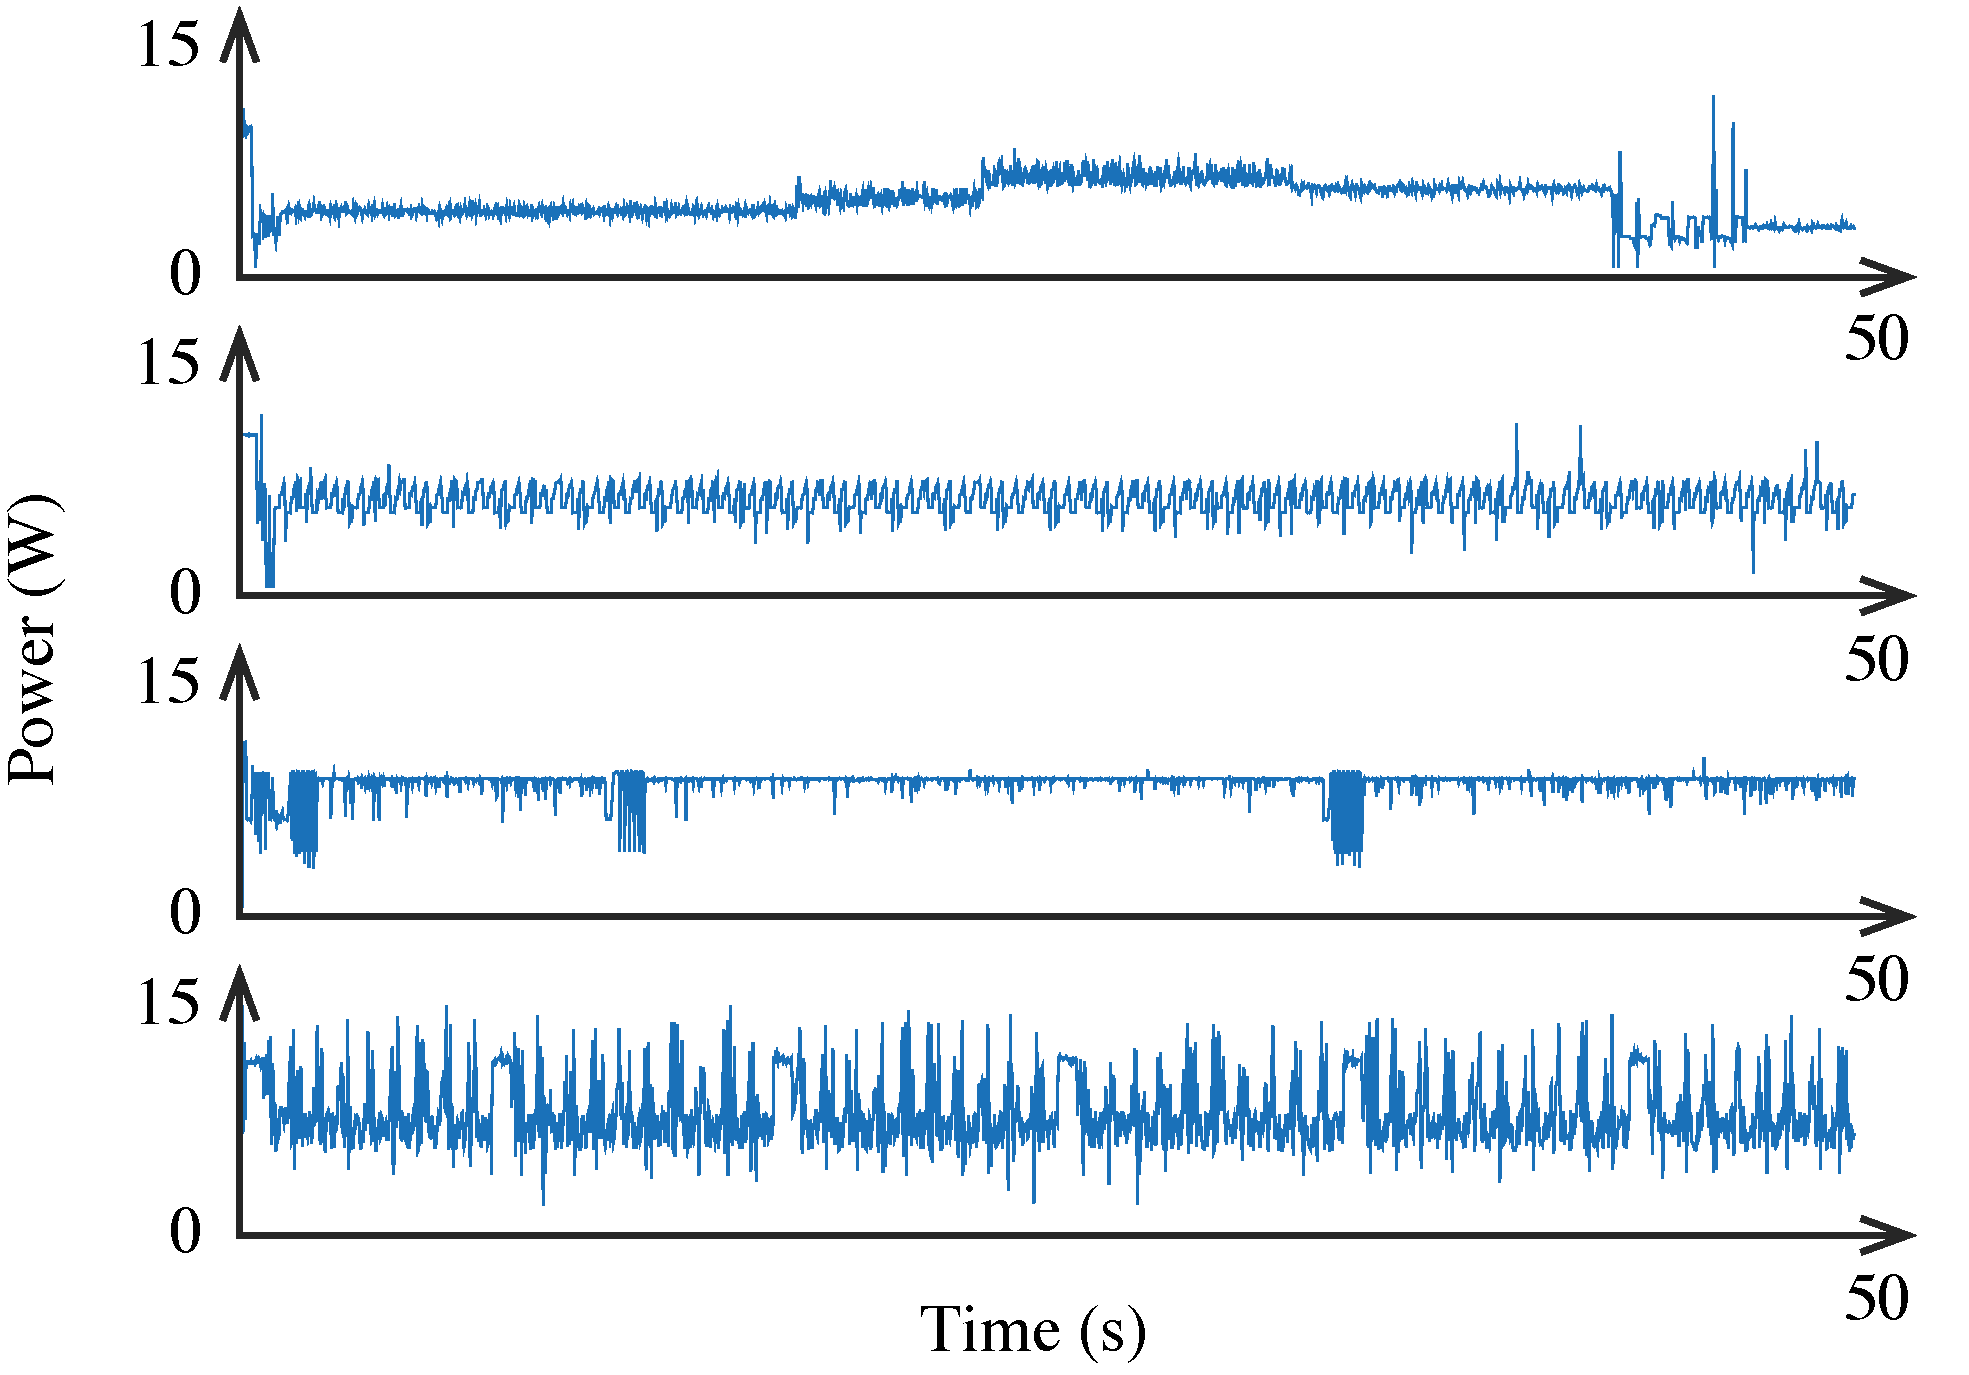
\includegraphics[width=1.0\columnwidth]{include/assets/figures/workload.pdf}
  \caption{
    Power traces of four applications from the \sc{SPEC CPU2006} benchmark
    suite, namely, \tt{astar}, \tt{GemsFDTD}, \tt{bwaves}, and \tt{wrf},
    respectively.
  }
  \flab{workload}
\end{figure}

In the previous subsection, we introduced our approach to generating streams of
arrivals; however, an arrival is only a time stamp without any information about
the actual workload. In this subsection, we describe how workloads needed for
substantiating job arrivals are obtained, which is depicted at the bottom of
\fref{methodology}. To begin with, workload candidates should conform to a
number of criteria. First, as emphasized throughout the paper, we aim to produce
realistic power and temperature traces, and, therefore, workloads should
represent well the applications or services that the system in question is
supposed to provide to the end user. Second, a workload should be fast to
evaluate, which, in our context, refers to obtaining the power consumption of
that workload.

The particularities of the power consumption of a computer program are hard to
fabricate. A sequence of random numbers taken out of thin air will not do the
trick as programs have certain algorithmic structures.
Figure~\ref{fig:workload} illustrates the power consumption of four applications
taken from the \sc{SPEC CPU2006} benchmark suite \cite{cpu2006}. A program
might, for instance, traverse a number of phases, and each phase might trigger a
number of distinctive computations, shaping the corresponding power and
temperature profiles. Such features are important to preserve in order to make
the subsequent experimentation with machine-learning techniques meaningful.

The workload modeling is based on full-system simulations of reference programs.
However, if we had incorporated such simulations directly into our workflow, it
would have defeated the purpose of our work since, as motivated in
\sref{motivation}, detailed simulations are too time consuming. Instead, we
propose the use of high-level recordings; see the modules labeled ``Recorder''
in \fref{methodology}. To elaborate, using an adequate simulator capable of
modeling the target architecture, we execute each reference program in isolation
and record certain information about this execution.\footnote{Such a technique
is similar in spirit to PinPlay \cite{patil2010}, which is a tool for recording
and replaying an execution of a program at the instruction level.} At a later
stage of our pipeline (see the module labeled ``Streamer'' in
\fref{methodology}), the collected information is utilized in order to flesh out
jobs upon their arrival, and this stage requires no simulation. These primitives
are building blocks: they are combined to form complex workloads corresponding
to multiple programs running in parallel, which will be further elaborated on in
\sref{composition}.

From our experience, performance and power simulation takes by far the largest
expense in terms of time, and, therefore, we propose to record power directly,
eliminating this expense all together. To this end, one first has to decide on a
time step, granularity level, and resource availability. The time step (sampling
interval) is exactly what it sounds. The granularity level specifies what parts
of the system are treated as recording locations. To give an example, one can
choose to track the power consumption of a core as a whole or opt for tracking
\sc{ALU}, \sc{FPU}, and so on individually. The resource availability defines
what computational resources are at a program's disposal. For instance, a
multithreaded program can be recorded as running on one core or several cores.

The result of the procedure is a repository of power traces corresponding to
real programs, which we refer to as workload patterns; see the bottom cloud in
\fref{methodology}. Note that, since a reference program can be recorded
differently---for instance, with different numbers of cores---it can potentially
have multiple entries in the repository. It is also worth noting that dynamic
and static power can be recorded separately in order to get a better control
over the subsequent composition.

Full-system simulations obviously take time; however, they should be done only
once. Moreover, since researchers tend to test their ideas using similar sets of
benchmark suites and considering similar sets of target architectures, it makes
sense to create a common repository of power patterns that will be populated and
maintained online by the research community. The repository could be structured
in a way that would allow for a proper accommodation of different target
architectures and other recording conditions. Having established such a common
repository, power patterns will be at a one-click distance from any single
researcher, and no prior simulation will be needed. The role of the repository
could be similar to the one played nowadays by the benchmark suites themselves,
but it would be on a different level of abstraction and for a different purpose.

Let us now turn to the question: How do we choose which workload pattern to use
for a particular arrival? First of all, since arrivals are modeled as a stream,
it is convenient to turn workloads into a stream as well so that we can draw an
element from each stream and obtain a fully characterized job (time and
payload). Then the question boils down to the logic behind the workload stream.
The workload stream can be dependent on the arrival stream, which allows for
modeling, for instance, periodic workloads. The workload stream can also be
autocorrelated, which allows for modeling, for instance, coupled workloads.
Since such aspects rely heavily on domain-specific knowledge, we refrain from
providing any particular dependency model. The default option used in our
toolchain, which is to be discussed in \sref{toolchain}, is drawing samples from
a uniform distribution over a set of workload patterns.

The stream abstraction introduced in the previous paragraph also helps to
communicate the notion of workload transformation. A workload transformation is
an optional operation that can be used for workload diversification and for
emulation of the effects of such techniques as dynamic voltage/frequency
scaling. A selected workload pattern can pass through a number of filters---such
as noise, offset, scale, stretch, and shrink---before being pulled from the
stream. This, however, should be done thoughtfully as the purpose of recording
power patterns is in part to bring in realistic power fluctuations.

To recapitulate, we have obtained a database of reference workloads and
discussed the formation of workload streams, which complement arrival streams.
The patterns correspond to executions of real programs and, thus, exhibit
realistic traits.
